\documentclass[10pt, reqno, letterpaper, twoside]{amsart}
\usepackage[margin=1in]{geometry}

\usepackage{amssymb, bm, mathtools}
\usepackage[usenames,dvipsnames,svgnames,table]{xcolor}
\usepackage[pdftex, xetex]{graphicx}
\usepackage{enumerate, setspace}
\usepackage{float, colortbl, tabularx, longtable, multirow, subcaption, environ, wrapfig, textcomp, booktabs}
\usepackage{pgf, tikz, framed, url, hyperref}
\usepackage[normalem]{ulem}
% \usetikzlibrary{arrows,positioning,automata,shadows,fit,shapes}
\usepackage[english]{babel}

\usepackage{microtype}
\microtypecontext{spacing=nonfrench}

\usepackage{times}
\usepackage[numbers,sort&compress]{natbib}

\usetikzlibrary{arrows.meta, positioning, fit, shapes.misc}
\tikzset{
  box/.style={draw, rounded corners, align=center, inner sep=6pt, minimum width=2.6cm, minimum height=1.0cm},
  sbox/.style={draw, rounded corners, align=center, inner sep=5pt, minimum width=2.4cm, minimum height=0.85cm},
  line/.style={-Latex, thick},
  dashedline/.style={-Latex, thick, dashed},
  note/.style={align=left, font=\small}
}

\title{Circuit Distillation for Math Reasoning: Aligning Computational Mechanisms in Large Language Models}
\author{
Eshan Singhal [esinghal@seas], Audhav Durai [audhav@wharton], \\ Vedant Gaur [vedantg@wharton], Praneel Varshney [pvarsh@seas]
}

\begin{document}

\begin{abstract}
    \emph{Circuit Distillation} is a mechanism-level method for transferring knowledge from a large teacher model to a smaller student model by aligning internal computational circuits rather than matching outputs, as is done in traditional knowledge distillation. We apply this approach to arithmetic reasoning in the Llama~3 family with a novel method that has a two-stage pipeline. First, we discover arithmetic-relevant circuits in the teacher using a classifier-based framework that clusters arithmetic problems into latent classes and learns sparse, mutually distinct, and functionally selective neuron-level masks for each class. Second, we distill these circuits into the student by enforcing mechanism-level alignment through representational similarity objectives. 

    \textbf{[Add 2-3 sentences of results here]}
\end{abstract}

\maketitle

\section{Introduction}

Large language models (LLMs) exhibit strong arithmetic and symbolic reasoning abilities when scaled to tens of billions of parameters \citep{dubey2024llama}. However, deploying such models is often infeasible due to computational and memory constraints. Knowledge distillation aims to address this by transferring capabilities from large teacher models to smaller student models, but conventional approaches focus on matching outputs rather than internal computation. As a result, distilled models often produce correct answers while relying on brittle heuristics rather than the teacher’s underlying algorithmic mechanisms \citep{wadhwa2024mysteries}.

Mechanistic interpretability suggests that many reasoning behaviors in transformers are implemented by sparse, functionally specialized subcircuits composed of particular neurons and attention heads \citep{elhage2021mathematical}. This motivates the question: \emph{can we identify such circuits and distill them directly into smaller models?} If so, student models could inherit not just surface-level behavior but the teacher’s internal reasoning process.

In this work, we focus on arithmetic reasoning and propose a neuron-level circuit discovery and distillation framework. We introduce a method that (i) clusters arithmetic problems into latent classes, (ii) learns sparse neuron masks for each class using a structured optimization objective, and (iii) uses these masks as the basis for circuit-level distillation that leverages representational similarity alignment between teacher and student \citep{kornblith2019similarity,williams2025equivalence}. Our approach emphasizes generality. That is, as long as the number of latent classes is sufficiently large to capture meaningful structure, the precise value of this hyperparameter is not critical.

\subsection{Contributions}

\begin{itemize}
\item We propose a neuron-level circuit discovery framework for arithmetic reasoning that jointly clusters problems and learns sparse neuron masks corresponding to each cluster.
\item We introduce a multi-term objective that enforces sparsity, balanced usage, and orthogonality between discovered circuits, yielding interpretable and functionally distinct neuron groups.
\item We apply this framework to both 1B- and 8B-parameter transformer models, demonstrating consistent circuit structure across scales.
\item We outline how the discovered circuits can be integrated into a circuit distillation pipeline for mechanism-level transfer using representational similarity objectives.
\end{itemize}

\section{Background}

\subsection{Transformers and Arithmetic}

Transformers process input sequences through layers of self-attention and feedforward networks (FFNs), producing intermediate activations that can be interpreted as contributing to the model’s computation \citep{elhage2021mathematical}. Arithmetic problems typically consist of fixed-length token sequences (e.g., three tokens for operands and two for operators), yielding structured activation patterns across layers.

\subsection{Neuron Masks as Circuits}

We model a circuit as a \emph{neuron mask}: a vector of weights applied multiplicatively to neuron outputs in FFN layers. This view aligns with research that circuits in transformers can be viewed as sparse subgraphs of the model’s computational graph responsible for particular behaviors \citep{elhage2021mathematical,wadhwa2025circuit}. Learning such masks facilitates both interpretability and targeted interventions.

\subsection{Representational Similarity}

Matching student and teacher representations using metrics invariant to orthogonal transformations, such as Centered Kernel Alignment (CKA), has proven effective for comparing internal states of models with different architectures \citep{kornblith2019similarity,williams2025equivalence}. We leverage this in the distillation objective to align circuit activations across student and teacher.

\section{Related Work}

\textbf{Knowledge Distillation.} Traditional distillation matches teacher and student output distributions and, in some cases, intermediate representations. However, these approaches do not explicitly transfer internal reasoning mechanisms. Chain-of-thought distillation has been proposed to include teacher rationales, but students may imitate style without acquiring causal computation \citep{wadhwa2024mysteries}.

\textbf{Mechanistic Interpretability and Circuits.} Mechanistic interpretability aims to decompose networks into interpretable components such as attention heads and neurons implementing specific functions. The transformer circuits paradigm formalizes this view, identifying subnetworks responsible for tasks like induction and arithmetic reasoning \citep{elhage2021mathematical}. Attribution Patching provides a scalable approximation for estimating component importance \citep{nanda2023attribution,kramar2024atp}.

\textbf{Similarity Metrics.} Centered Kernel Alignment (CKA) has emerged as a robust method for comparing representations across models, due to its invariance to invertible linear transformations and stability in high dimensions \citep{kornblith2019similarity,williams2025equivalence}.

\section{Approach}

Our circuit discovery framework consists of three components: problem encoding and clustering, neuron mask generation, and a multi-term optimization objective that enforces interpretability and functional separation.

\subsection{Problem Encoding and Latent Classes}

Given an arithmetic problem \(x_i\), we compute a fixed-dimensional problem encoding using intermediate transformer activations. This encoding is passed to a \(K\)-class classifier, where \(K\) is a user-specified hyperparameter controlling the granularity of discovered circuits. The classifier’s output distribution is sampled via Gumbel-Softmax with a straight-through estimator to facilitate end-to-end gradients while yielding discrete class assignments.

\subsection{Neuron Mask Generator}

Conditioned on the sampled class, a two-layer feedforward network produces a neuron mask \(\mathbf{m}_k \in (0,1)^D\), where \(D\) is the number of neurons in the target FFN layers. Each mask weight modulates the corresponding neuron activation via elementwise multiplication. Masks are shared across all problems assigned to the same class, encouraging each class to correspond to a consistent computational subcircuit.

\subsection{Objective Function}

We introduce the following notation:

\begin{itemize}
\item \(K\): number of latent problem classes.
\item \(i \in \{1,\dots,N_k\}\): index over problems assigned to class \(k\).
\item \(d \in \{1,\dots,D\}\): neuron index.
\item \(a_{i,k,d}\): activation of neuron \(d\) for problem \(i\) in class \(k\).
\item \(m_{k,d}\): neuron mask weight for neuron \(d\) in class \(k\).
\item \(\mathbf{M}_k \in \mathbb{R}^D\): mask vector for class \(k\).
\item \(f_k\): empirical probability that class \(k\) is selected.
\item \(\pi\): target average mask activation (e.g., \(0.1\)).
\end{itemize}

The total loss is:

\[
\mathcal{L}
= \lambda_1 \mathcal{L}_{\text{sim}}
+ \lambda_2 \mathcal{L}_{\text{usage}}
+ \lambda_3 \mathcal{L}_{\text{sparsity}}
+ \lambda_4 \mathcal{L}_{\text{KL}}
+ \lambda_5 \mathcal{L}_{\text{mask-sim}}.
\]

\subsubsection{Similarity Loss}

\[
\mathcal{L}_{\text{sim}}
= -\frac{1}{K}
\sum_{k=1}^{K}
\frac{1}{N_k (N_k - 1)}
\sum_{d=1}^{D}
\left(
\sum_{i=1}^{N_k} \lVert a_{i,k,d} \rVert
\right)^2.
\]

\subsubsection{Usage Entropy}

\[
\mathcal{L}_{\text{usage}}
= - \sum_{k=1}^{K} f_k \log f_k.
\]

\subsubsection{Sparsity Loss}

\[
\mathcal{L}_{\text{sparsity}}
= -\frac{1}{K}
\sum_{k=1}^{K}
\frac{1}{D}
\sum_{d=1}^{D}
\left[
m_{k,d} \log m_{k,d}
+ (1 - m_{k,d}) \log (1 - m_{k,d})
\right].
\]

\subsubsection{KL Regularization}

\[
\mathcal{L}_{\text{KL}}
= \bar{m} \log \frac{\bar{m}}{\pi}
+ (1 - \bar{m}) \log \frac{1 - \bar{m}}{1 - \pi},
\quad
\bar{m} = \frac{1}{KD} \sum_{k,d} m_{k,d}.
\]

\subsubsection{Mask Orthogonality Loss}

\[
\mathcal{L}_{\text{mask-sim}}
= \frac{1}{K(K-1)}
\sum_{k_1=1}^{K}
\sum_{\substack{k_2=1 \\ k_2 \neq k_1}}^{K}
\mathbf{M}_{k_1}^\top \mathbf{M}_{k_2}.
\]

\subsection{Circuit Discovery Model Architecture}
We learn a latent-class circuit decomposition over arithmetic problems and use it to generate sparse neuron-level masks over MLP activations. Given an equation $x$ (e.g., $12+34=46$), we parse the operands and result $(o_1,o_2,r)$ and embed them with a lightweight \emph{ProblemEncoder} that concatenates learned embeddings for $o_1$, $o_2$, and $r$ into a fixed-dimensional vector $\phi(x)$.

A small MLP classifier maps $\phi(x)$ to logits over $K$ latent classes, and we sample a discrete class assignment using straight-through Gumbel-Softmax. Conditioned on the sampled class, we generate neuron masks separately for the 1B and 8B models. Each mask generator is a compact network (class embedding $\rightarrow$ linear $\rightarrow$ sigmoid) that outputs a mask vector $\mathbf{m}\in(0,1)^D$, where $D=\texttt{intermediate\_size}\times\texttt{num\_hidden\_layers}$ corresponds to flattened MLP neurons across all transformer blocks. The mask is applied multiplicatively to the stacked per-layer MLP activations.

We optimize a multi-term objective that (i) increases within-class similarity of masked activations, (ii) encourages sparse/binary masks via entropy and a global Bernoulli KL-to-prior term, (iii) discourages overlap between class masks via mean pairwise cosine similarity, and (iv) encourages balanced class usage via an entropy bonus.

\subsubsection{Circuit Discovery Training Dynamics}
We analyze the optimization behavior of the circuit discovery objective to verify that it produces sparse, distinct, and functionally meaningful neuron masks. First, the sparsity-related terms jointly encourage masks with a controlled activation budget: the binary-entropy sparsity loss drives mask entries toward near-binary values, while the KL regularization term constrains the global mean activation rate toward a Bernoulli prior with $\pi=0.1$. As training progresses, these terms decrease in tandem, indicating convergence to sparse masks with approximately 10\% active neurons. 

Second, we examine the interaction between representativeness and separation of discovered circuits. The within-class similarity objective encourages masked activations corresponding to the same latent class to be consistent, while the mask cosine similarity penalty discourages overlap between class-conditioned masks. Over training, similarity improves as mask cosine similarity decreases, suggesting that the learned circuits become both representative of their assigned problem classes and increasingly orthogonal to one another. See Appendix~\ref{app:training-dynamics} for training curves.



\begin{thebibliography}{99}

\bibitem{dubey2024llama}
Abhimanyu Dubey, Abhinav Jauhri, Abhinav Pandey, and others.
\newblock The Llama 3 Herd of Models.
\newblock \emph{arXiv preprint arXiv:2407.21783}, 2024.

\bibitem{wadhwa2025circuit}
Somin Wadhwa, Silvio Amir, and Byron C. Wallace.
\newblock Circuit Distillation.
\newblock \emph{arXiv preprint arXiv:2509.25002}, 2025.

\bibitem{wadhwa2024mysteries}
Somin Wadhwa, Silvio Amir, and Byron C. Wallace.
\newblock Investigating mysteries of CoT-augmented distillation.
\newblock In \emph{Proceedings of the 2024 Conference on Empirical Methods in Natural Language Processing}, pages 6071--6086, 2024.

\bibitem{elhage2021mathematical}
Nelson Elhage, Neel Nanda, Catherine Olsson, and others.
\newblock A Mathematical Framework for Transformer Circuits.
\newblock \emph{Transformer Circuits Thread}, 2021.

\bibitem{nanda2023attribution}
Neel Nanda.
\newblock Attribution Patching: Activation Patching at Industrial Scale.
\newblock 2023.

\bibitem{kramar2024atp}
János Kramár, Tom Lieberum, Rohin Shah, and Neel Nanda.
\newblock AtP*: An efficient and scalable method for localizing LLM behaviour to components.
\newblock \emph{arXiv preprint arXiv:2403.00745}, 2024.

\bibitem{mueller2025mib}
Aaron Mueller and others.
\newblock MIB: A Mechanistic Interpretability Benchmark.
\newblock \emph{arXiv preprint arXiv:2504.13151}, 2025.

\bibitem{kornblith2019similarity}
Simon Kornblith, Mohammad Norouzi, Honglak Lee, and Geoffrey Hinton.
\newblock Similarity of Neural Network Representations Revisited.
\newblock In \emph{International Conference on Machine Learning}, 2019.

\bibitem{williams2025equivalence}
Alex Williams and others.
\newblock An Equivalence Between Representational Similarity Analysis and Centered Kernel Alignment.
\newblock \emph{Cognitive Computational Neuroscience}, 2025.

\end{thebibliography}

\clearpage
\appendix

\section{Additional Figures}
\label{app:additional-figures}
\subsection{Circuit Discovery Architecture}


\begin{figure}[b]
    \centering
    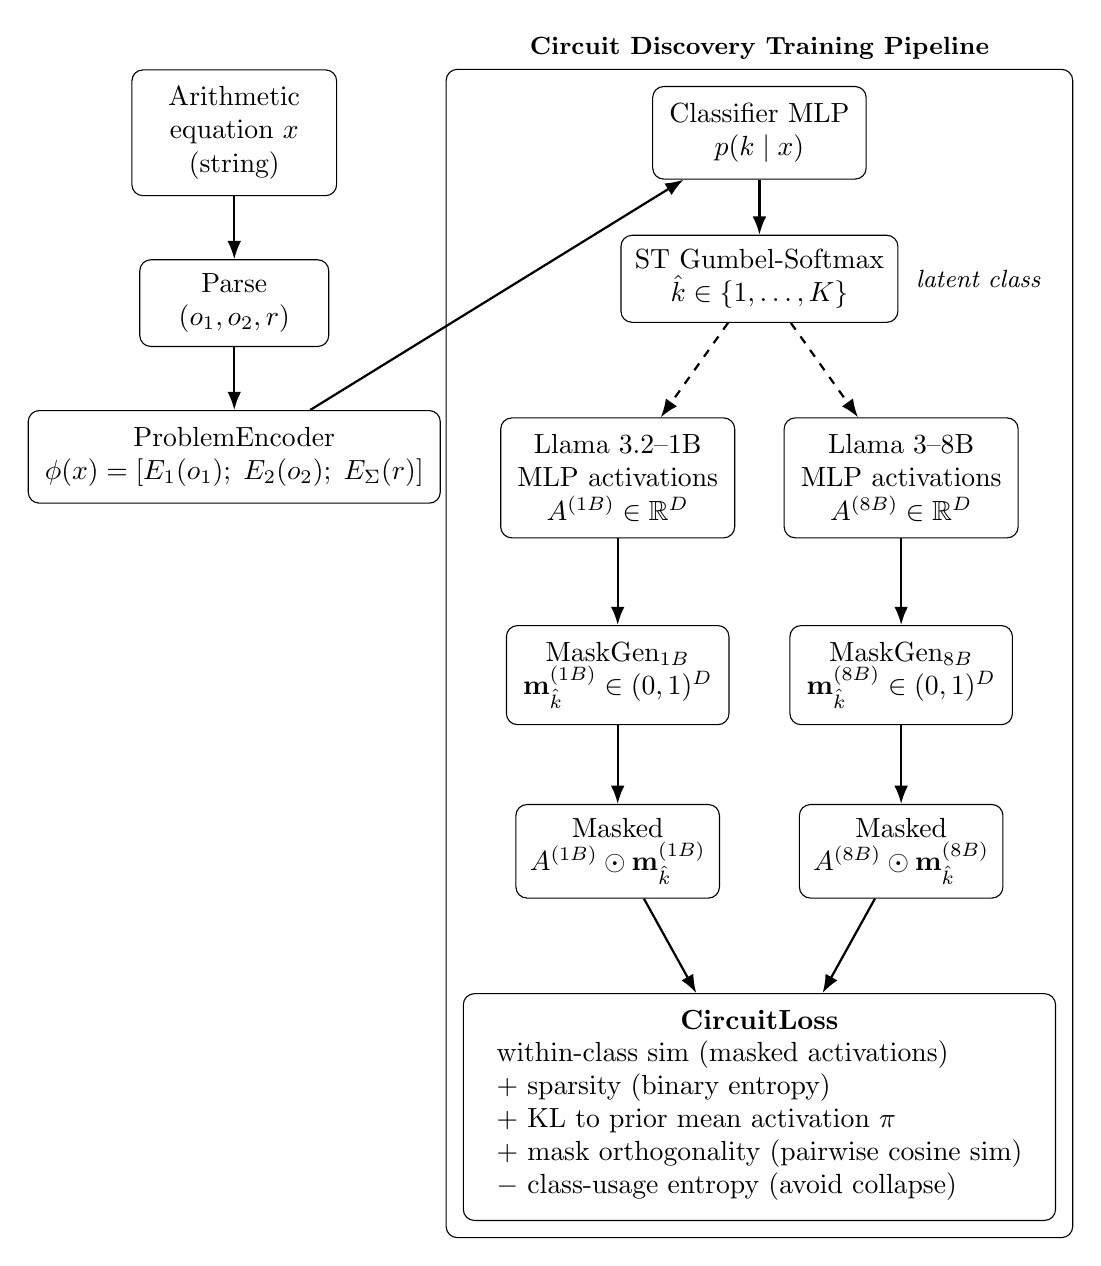
\begin{tikzpicture}[node distance=1.0cm and 1.5cm]
    
    \node[box] (eq) {Arithmetic\\equation $x$\\(string)};
    \node[sbox, below=0.8cm of eq] (parse) {Parse\\$(o_1,o_2,r)$};
    \node[box, below=0.8cm of parse] (enc) {ProblemEncoder\\
    $\phi(x)=[E_1(o_1);\;E_2(o_2);\;E_\Sigma(r)]$};
    
    \node[box, right=4.0cm of eq] (clf) {Classifier MLP\\$p(k\mid x)$};
    \node[sbox, below=0.7cm of clf] (gumbel) {ST Gumbel-Softmax\\$\hat{k}\in\{1,\dots,K\}$};
    \node[note, right=0.1cm of gumbel] {\emph{latent class}};
    
    \node[box, below=1.2cm of gumbel, xshift=-1.8cm] (acts1b) {Llama 3.2--1B\\MLP activations\\$A^{(1B)}\in\mathbb{R}^{D}$};
    \node[box, below=1.2cm of gumbel, xshift=1.8cm] (acts8b) {Llama 3--8B\\MLP activations\\$A^{(8B)}\in\mathbb{R}^{D}$};
    
    \node[box, below=1.1cm of acts1b] (mask1b) {MaskGen$_{1B}$\\
    $\mathbf{m}^{(1B)}_{\hat{k}}\in(0,1)^{D}$};
    \node[box, below=1.1cm of acts8b] (mask8b) {MaskGen$_{8B}$\\
    $\mathbf{m}^{(8B)}_{\hat{k}}\in(0,1)^{D}$};
    
    \node[sbox, below=1.0cm of mask1b] (masked1b) {Masked\\$A^{(1B)}\odot \mathbf{m}^{(1B)}_{\hat{k}}$};
    \node[sbox, below=1.0cm of mask8b] (masked8b) {Masked\\$A^{(8B)}\odot \mathbf{m}^{(8B)}_{\hat{k}}$};
    
    \node[box, below=1.2cm of masked1b, xshift=1.8cm, minimum width=5.5cm] (loss) {
    \textbf{CircuitLoss}\\[2pt]
    \begin{tabular}{l}
    within-class sim (masked activations)\\
    + sparsity (binary entropy)\\
    + KL to prior mean activation $\pi$\\
    + mask orthogonality (pairwise cosine sim)\\
    $-$ class-usage entropy (avoid collapse)
    \end{tabular}
    };
    
    \draw[line] (eq) -- (parse);
    \draw[line] (parse) -- (enc);
    \draw[line] (enc) -- (clf);
    \draw[line] (clf) -- (gumbel);
    
    \draw[dashedline] (gumbel) -- (acts1b);
    \draw[dashedline] (gumbel) -- (acts8b);
    
    \draw[line] (acts1b) -- (mask1b);
    \draw[line] (acts8b) -- (mask8b);
    
    \draw[line] (mask1b) -- (masked1b);
    \draw[line] (mask8b) -- (masked8b);
    
    \draw[line] (masked1b) -- (loss);
    \draw[line] (masked8b) -- (loss);
    
    \node[draw, rounded corners, inner sep=6pt, fit=(clf) (gumbel) (acts1b) (acts8b) (mask1b) (mask8b) (masked1b) (masked8b) (loss),
    label={[font=\small]above:\textbf{Circuit Discovery Training Pipeline}}] (fitbox) {};
    
    \end{tikzpicture}
    \caption{Circuit discovery architecture. Problems are embedded and assigned to a latent class via a straight-through Gumbel-Softmax classifier. The sampled class selects a class-conditioned neuron mask for each teacher model (1B and 8B), which gates flattened MLP activations. Training optimizes a multi-term objective encouraging within-class functional similarity, sparse masks, distinct circuits, and balanced class usage.}
    \label{fig:circuit-discovery-arch}
\end{figure}

\section{Circuit Discovery Training Dynamics}
\label{app:training-dynamics}

\begin{figure}[H]
    \centering
    \includegraphics[width=0.92\linewidth]{figures/cd_sparsify.png}
    \caption{Circuit discovery training curves related to sparsity regularization (binary-entropy sparsity loss and KL-to-prior mean activation). These curves support the discussion in Section~4.5.}
    \label{fig:cd-training-sparsity}
\end{figure}

\begin{figure}[H]
    \centering
    \includegraphics[width=0.92\linewidth]{figures/cd_rep_ortho.png}
    \caption{Circuit discovery training curves related to representativeness (within-class similarity) and separation (mask orthogonality / cosine similarity). These curves support the discussion in Section~4.5.}
    \label{fig:cd-training-rep-ortho}
\end{figure}

\end{document}
